
\subsection{Braiding cube commutes}
In this section we show that the braiding cube \autoref{bradingcube} given by the extended Waldhausen construction always commutes.

The source for this cube is the following cube in $\OrdSet\otimes\OrdSet$ (described in \cite[\S3.4]{GGSSH}):
\[
C=\left(\stik{0.8}{
 \& \ord{3} \ar{rr} \ar{dd} \& {} \& \ord{2} \ar{dd}\\
\ord{3} \ar[crossing over]{rr} \ar{dd} \ar[equal]{ur} \& {} \& \ord{2} \ar{dd} \ar[equal]{ur}\& {}\\
{} \& \ord{2} \ar{rr} \& {} \& \ord{1}\\
\ord{2} \ar{rr} \ar[equal]{ur} \& {} \& \ord{1} \ar[equal]{ur}
\latearrow{commutative diagrams/crossing over}{2-3}{4-3}{}
}
,
\stik{0.8}{
 \& \ord{1} \ar[equal]{rr} \ar[equal]{dd} \& {} \& \ord{1} \ar[equal]{dd}\\
\ord{2} \ar[crossing over,equal]{rr} \ar[equal]{dd} \ar{ur} \& {} \& \ord{2} \ar[equal]{dd} \ar{ur}\& {}\\
{} \& \ord{1} \ar[equal]{rr} \& {} \& \ord{1}\\
\ord{2} \ar[equal]{rr} \ar{ur} \& {} \& \ord{2} \ar{ur}
\latearrow{commutative diagrams/crossing over,commutative diagrams/equal}{2-3}{4-3}{}
}
\right)
\]
and it's image is a cube of spans in stacks, i.e. a $2\times 2 \times 2$ grid of cubes. To show that the image in categories is commutative, we need to show that the upper-right-back and lower-left-front cubes are pullbacks.

Using \cite[Lemma A.2]{GeometricHallAlgebra1} we need to show that two opposing faces in each cube are pullbacks.

Consider first the upper-right-back cube. Looking at the back face of $C$ we see that its back face is the upper-right square of the image of the associator square, which is a pullback as discussed in \cite{GeometricHallAlgebra1} (this is equivalent to part of the 2-Segal condition).

Therefore, we only need to show that its front face is a pullback. Let us consider the square in $\lSet$ giving rise to it:
\[
\stik{1}{
 \aug{\ord{2}\times\ord{2}}\sqcup\aug{\ord{2}} \dar \& \aug{\ord{2}}\sqcup\aug{\ord{2}} \lar \dar\\
 \aug{\ord{3}\times\ord{2}} \& \aug{\ord{2}\times\ord{2}} \lar
}
\]

The image of this in stacks, in pictorial terms (as in \autoref{BraidingHallAlgebra}), is:
\[
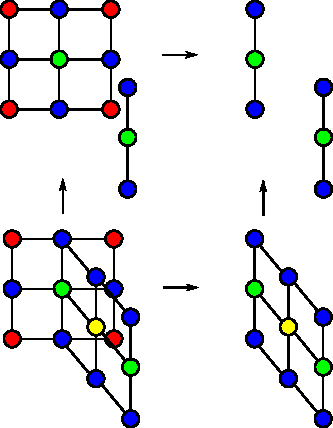
\includegraphics{Figures/HallBraidCubeURB-F.pdf}
\]

which is clearly a pullback square. The argument for the lower-left-front cube is almost identical.